\section{UDP Client - Server}
\subsection{Aim}
To implement Client-Server communication using Socket Programming and UDP as
transport layer protocol.

\subsection{Theory}
\textbf{UDP (User Datagram Protocol)} is an alternative communications protocol to
Transmission Control Protocol (TCP) used primarily for establishing low-latency
and loss-tolerating connections between applications on the internet. UDP enables
process-to-process communication. UDP sends messages, called datagrams, and is
considered a best-effort mode of communications. It is considered a connectionless
protocol because it doesn’t require a virtual circuit to be established before any data
transfer occurs.\\
\textbf{Server \& Client} - Since the UDP is a connectionless protocol, they do not require a connection 
to get established prior to data transmission or reception. Hence
data can be sent between them directly

\subsection{Algorithm}
\subsubsection{Server}
\begin{verbatim}
1 START
2 Create the UDP socket
3 Configure socket details
4 Bind the address struct to the socket using bind()
5 Recieve from client using recvfrom()
6 Print the recieved message
7 Send response using sento()
8 STOP
\end{verbatim}

\subsubsection{Client}
\begin{verbatim}
1 START
2 Create the socket using socket()
3 Configure the socket details
4 Send the message to the server using sendto()
5 Recieve the response from server using recvfrom()
6 Print the response
7 STOP
\end{verbatim}

\subsection{Source Code}
\subsubsection{Server}
\begin{lstlisting}[language=C]
  #include <stdio.h>
  #include <stdlib.h>
  #include <netinet/in.h>
  #include <sys/types.h>
  #include <sys/socket.h>
  #include <errno.h>
  #include <string.h>
  
  #define MESSAGE_SIZE 200
  
  typedef struct sockaddr sockaddr_t;
  typedef struct sockaddr_in sockaddr_in_t;
  
  extern int errno;
  
  const int PORT = 3000;
  
  void create_socket(int *socket_fd) {
    if((*socket_fd = socket(AF_INET, SOCK_DGRAM, 0)) == -1) {
      perror("Failed to create socket");
      fprintf(stderr, "Errno: %d\n", errno);
      exit(EXIT_FAILURE);
    }
  
    fprintf(stdout, "Socket created with UDP protocol\n");
  }
  
  void configure_socket(int *socket_fd) {
    sockaddr_in_t server_addr;
  
    server_addr.sin_family = AF_INET;
    server_addr.sin_port = PORT;
    server_addr.sin_addr.s_addr = htonl(INADDR_ANY);
  
    if(bind(*socket_fd, (sockaddr_t *)&server_addr, sizeof(server_addr)) == -1) {
      perror("Failed to bind socket configuration");
      fprintf(stderr, "Errno: %d\n", errno);
      exit(EXIT_FAILURE);
    }
  
    fprintf(stdout, "Socket binding successful\n");
  }
  
  void recieve_message(
    int *socket_fd, sockaddr_in_t *client_addr, unsigned int *client_addr_size
  ) {
    int message_length = 0;
    char message[MESSAGE_SIZE];
  
    fprintf(stdout, "Waiting for message from client\n");
  
    message_length = recvfrom(
      *socket_fd,
      (char *) message,
      MESSAGE_SIZE,
      MSG_WAITALL,
      (sockaddr_t *) client_addr,
      client_addr_size
    );
  
    message[message_length] = '\0';
    fprintf(stdout, "Message recieved from client: %s\n", message);
  }
  
  void send_acknowledgement(
    int *socket_fd, sockaddr_in_t *client_addr, unsigned int client_addr_size
  ) {
    const char *ack = "Message recieved successfully";
    size_t ack_size = strlen(ack);
  
    sendto(
      *socket_fd,
      ack,
      ack_size,
      MSG_CONFIRM,
      (sockaddr_t *) client_addr,
      client_addr_size
    );
  }
  
  int main() {
    int socket_fd;
    sockaddr_in_t client_addr; // Used to store client address
    unsigned int client_addr_size = sizeof(client_addr);
  
    create_socket(&socket_fd);
    configure_socket(&socket_fd);
    recieve_message(&socket_fd, &client_addr, &client_addr_size);
    send_acknowledgement(&socket_fd, &client_addr, client_addr_size);
  }
\end{lstlisting}

\subsubsection{Client}
\begin{lstlisting}[language=C]
  #include <stdio.h>
  #include <stdlib.h>
  #include <netinet/in.h>
  #include <sys/types.h>
  #include <sys/socket.h>
  #include <errno.h>
  #include <string.h>
  
  #define MESSAGE_SIZE 200
  
  typedef struct sockaddr sockaddr_t;
  typedef struct sockaddr_in sockaddr_in_t;
  
  extern int errno;
  
  const int PORT = 3000;
  
  void create_socket(int *socket_fd) {
    if((*socket_fd = socket(AF_INET, SOCK_DGRAM, 0)) == -1) {
      perror("Failed to create socket");
      fprintf(stderr, "Errno: %d\n", errno);
      exit(EXIT_FAILURE);
    }
  
    fprintf(stdout, "Socket created with UDP protocol\n");
  }
  
  void configure_server_info(
    sockaddr_in_t *server_addr, unsigned int server_addr_size
  ) {
    server_addr->sin_family = AF_INET;
    server_addr->sin_port = PORT;
    server_addr->sin_addr.s_addr = htonl(INADDR_ANY);
  
    fprintf(stdout, "Configuring server info successful\n");
  }
  
  void send_message(
    int *socket_fd, sockaddr_in_t *server_addr, unsigned int server_addr_size
  ) {
    const char *message = "Hello world";
    size_t message_size = strlen(message);
  
    sendto(
      *socket_fd,
      message,
      message_size,
      MSG_WAITALL,
      (sockaddr_t *) server_addr,
      server_addr_size
    );
  
    fprintf(stdout, "Message sent to server\n");
  }
  
  void recieve_acknowledgement(
    int *socket_fd, sockaddr_in_t *server_addr, unsigned int server_addr_size
  ) {
    int message_length = 0;
    char message[MESSAGE_SIZE];
  
    fprintf(stdout, "Waiting for acknowledgement from server\n");
  
    message_length = recvfrom(
      *socket_fd,
      (char *) message,
      MESSAGE_SIZE,
      MSG_CONFIRM,
      (sockaddr_t *) server_addr,
      &server_addr_size
    );
  
    message[message_length] = '\0';
    printf("Message recieved from server: %s\n", message);
  }
  
  
  int main() {
    int socket_fd;
    sockaddr_in_t socket_addr; // Used to store server address
    unsigned int socket_addr_size = sizeof(socket_addr);
  
    create_socket(&socket_fd);
    configure_server_info(&socket_addr, socket_addr_size);
    send_message(&socket_fd, &socket_addr, socket_addr_size);
    recieve_acknowledgement(&socket_fd, &socket_addr, socket_addr_size);
  }
\end{lstlisting}

\begin{center}
	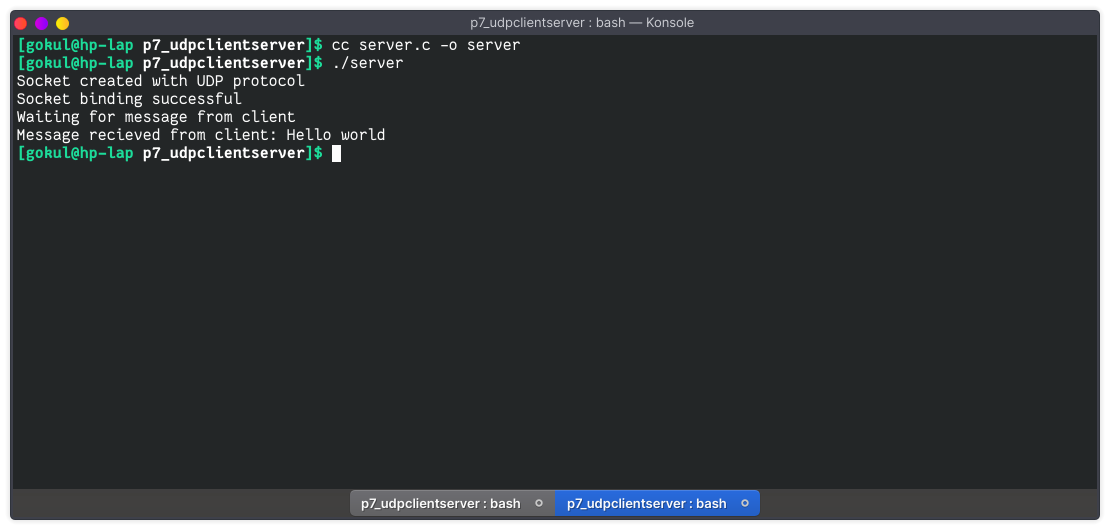
\includegraphics[width=0.90\textwidth]{img/p8/ss1.png}
	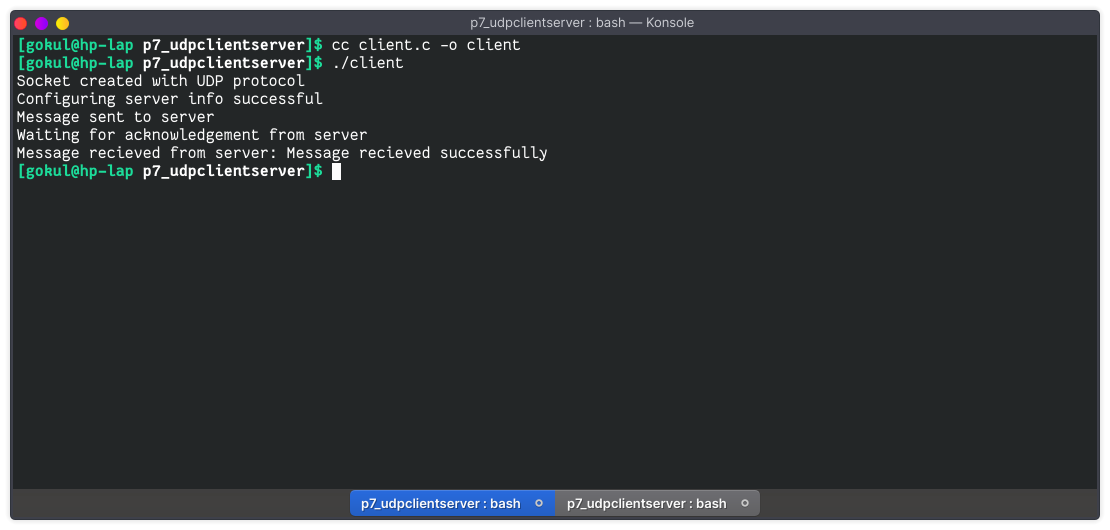
\includegraphics[width=0.90\textwidth]{img/p8/ss2.png}
\end{center}


\subsection{Result}
The above programs were executed and its output were verified